\section{Ergebnisse und Evaluation}
\label{sec:ergebnisse}

In diesem Kapitel wird die Leistungsfähigkeit der entwickelten Modelle auf dem finalen Testdatensatz (Januar 2022 bis August 2024) analysiert.
Die Evaluation erfolgt sowohl für klassische Machine-Learning-Verfahren als auch für Deep-Learning-Architekturen.

\subsection{Definition der Evaluationsmetriken}

Um die Vorhersagequalität objektiv zu bewerten, kommen verschiedene statistische Kennzahlen zum Einsatz, die unterschiedliche Aspekte des Modellverhaltens beleuchten:


\subsubsection{Mean Absolute Error (MAE)}
Dieser Wert gibt den durchschnittlichen Betrag der Abweichung zwischen Vorhersage und Realität an.
Er ist in der gleichen Einheit wie die Zielvariable (hier: Log-Returns) skaliert und lässt sich als "`durchschnittlicher Vorhersagefehler"' interpretieren.
Ein kleinerer Wert beweist eine höhere Präzision.

\subsubsection{Root Mean Squared Error (RMSE)} 
Im Vergleich zum MAE werden Fehler hier vor der Mittelwertbildung quadriert.
Dadurch werden größere Abweichungen (Ausreißer) stark gewichtet.
Für die Praxis bedeutet ein hoher RMSE bei gleichzeitig niedrigem MAE, dass das Modell zwar oft nah am Ziel liegt, aber gelegentlich sehr starke Fehlprognosen abgibt.

\subsubsection{Bestimmtheitsmaß ($R^2$)} 
Diese Kennzahl vergleicht die Varianz der Modellvorhersagen mit der Varianz der tatsächlichen Daten.
Ein $R^2$ von $1,0$ entspräche einer perfekten Vorhersage.
Ein $R^2$ nahe $0$ bedeutet, dass das Modell nicht besser ist als die einfache Vorhersage des historischen Mittelwertes.
Negative Werte indizieren, dass das Modell schlechter performt als dieser Mittelwert.

\subsubsection{Directional Accuracy (Richtungsgenauigkeit)} 
Für den praktischen Einsatz im Einkauf ist oft wichtiger zu wissen, ob der Preis steigt oder fällt, als den exakten Wert zu kennen.
Diese Metrik berechnet den prozentualen Anteil der korrekt vorhergesagten Richtungsänderungen.
Ein Wert von $50\,\%$ entspricht der Trefferquote eines reinen Zufallsprozesses, wie einem Münzwurf.

\subsubsection{Coverage@95\%} 
Diese Kennzahl gibt an, wie viel Prozent der tatsächlichen Werte innerhalb des vom Modell berechneten 95\%-Konfidenzintervalls liegen.
Bei einem perfekten Modell sollte dieser Wert exakt bei $95\,\%$ liegen.

\subsection{Vergleich der Basismodelle}
Abbildung \ref{fig:model_comp} zeigt die Performance verschiedener Modelle und Baselines für den nächsten Handelstag ($h=1$). 

\begin{figure}[hpt!]
\centering
	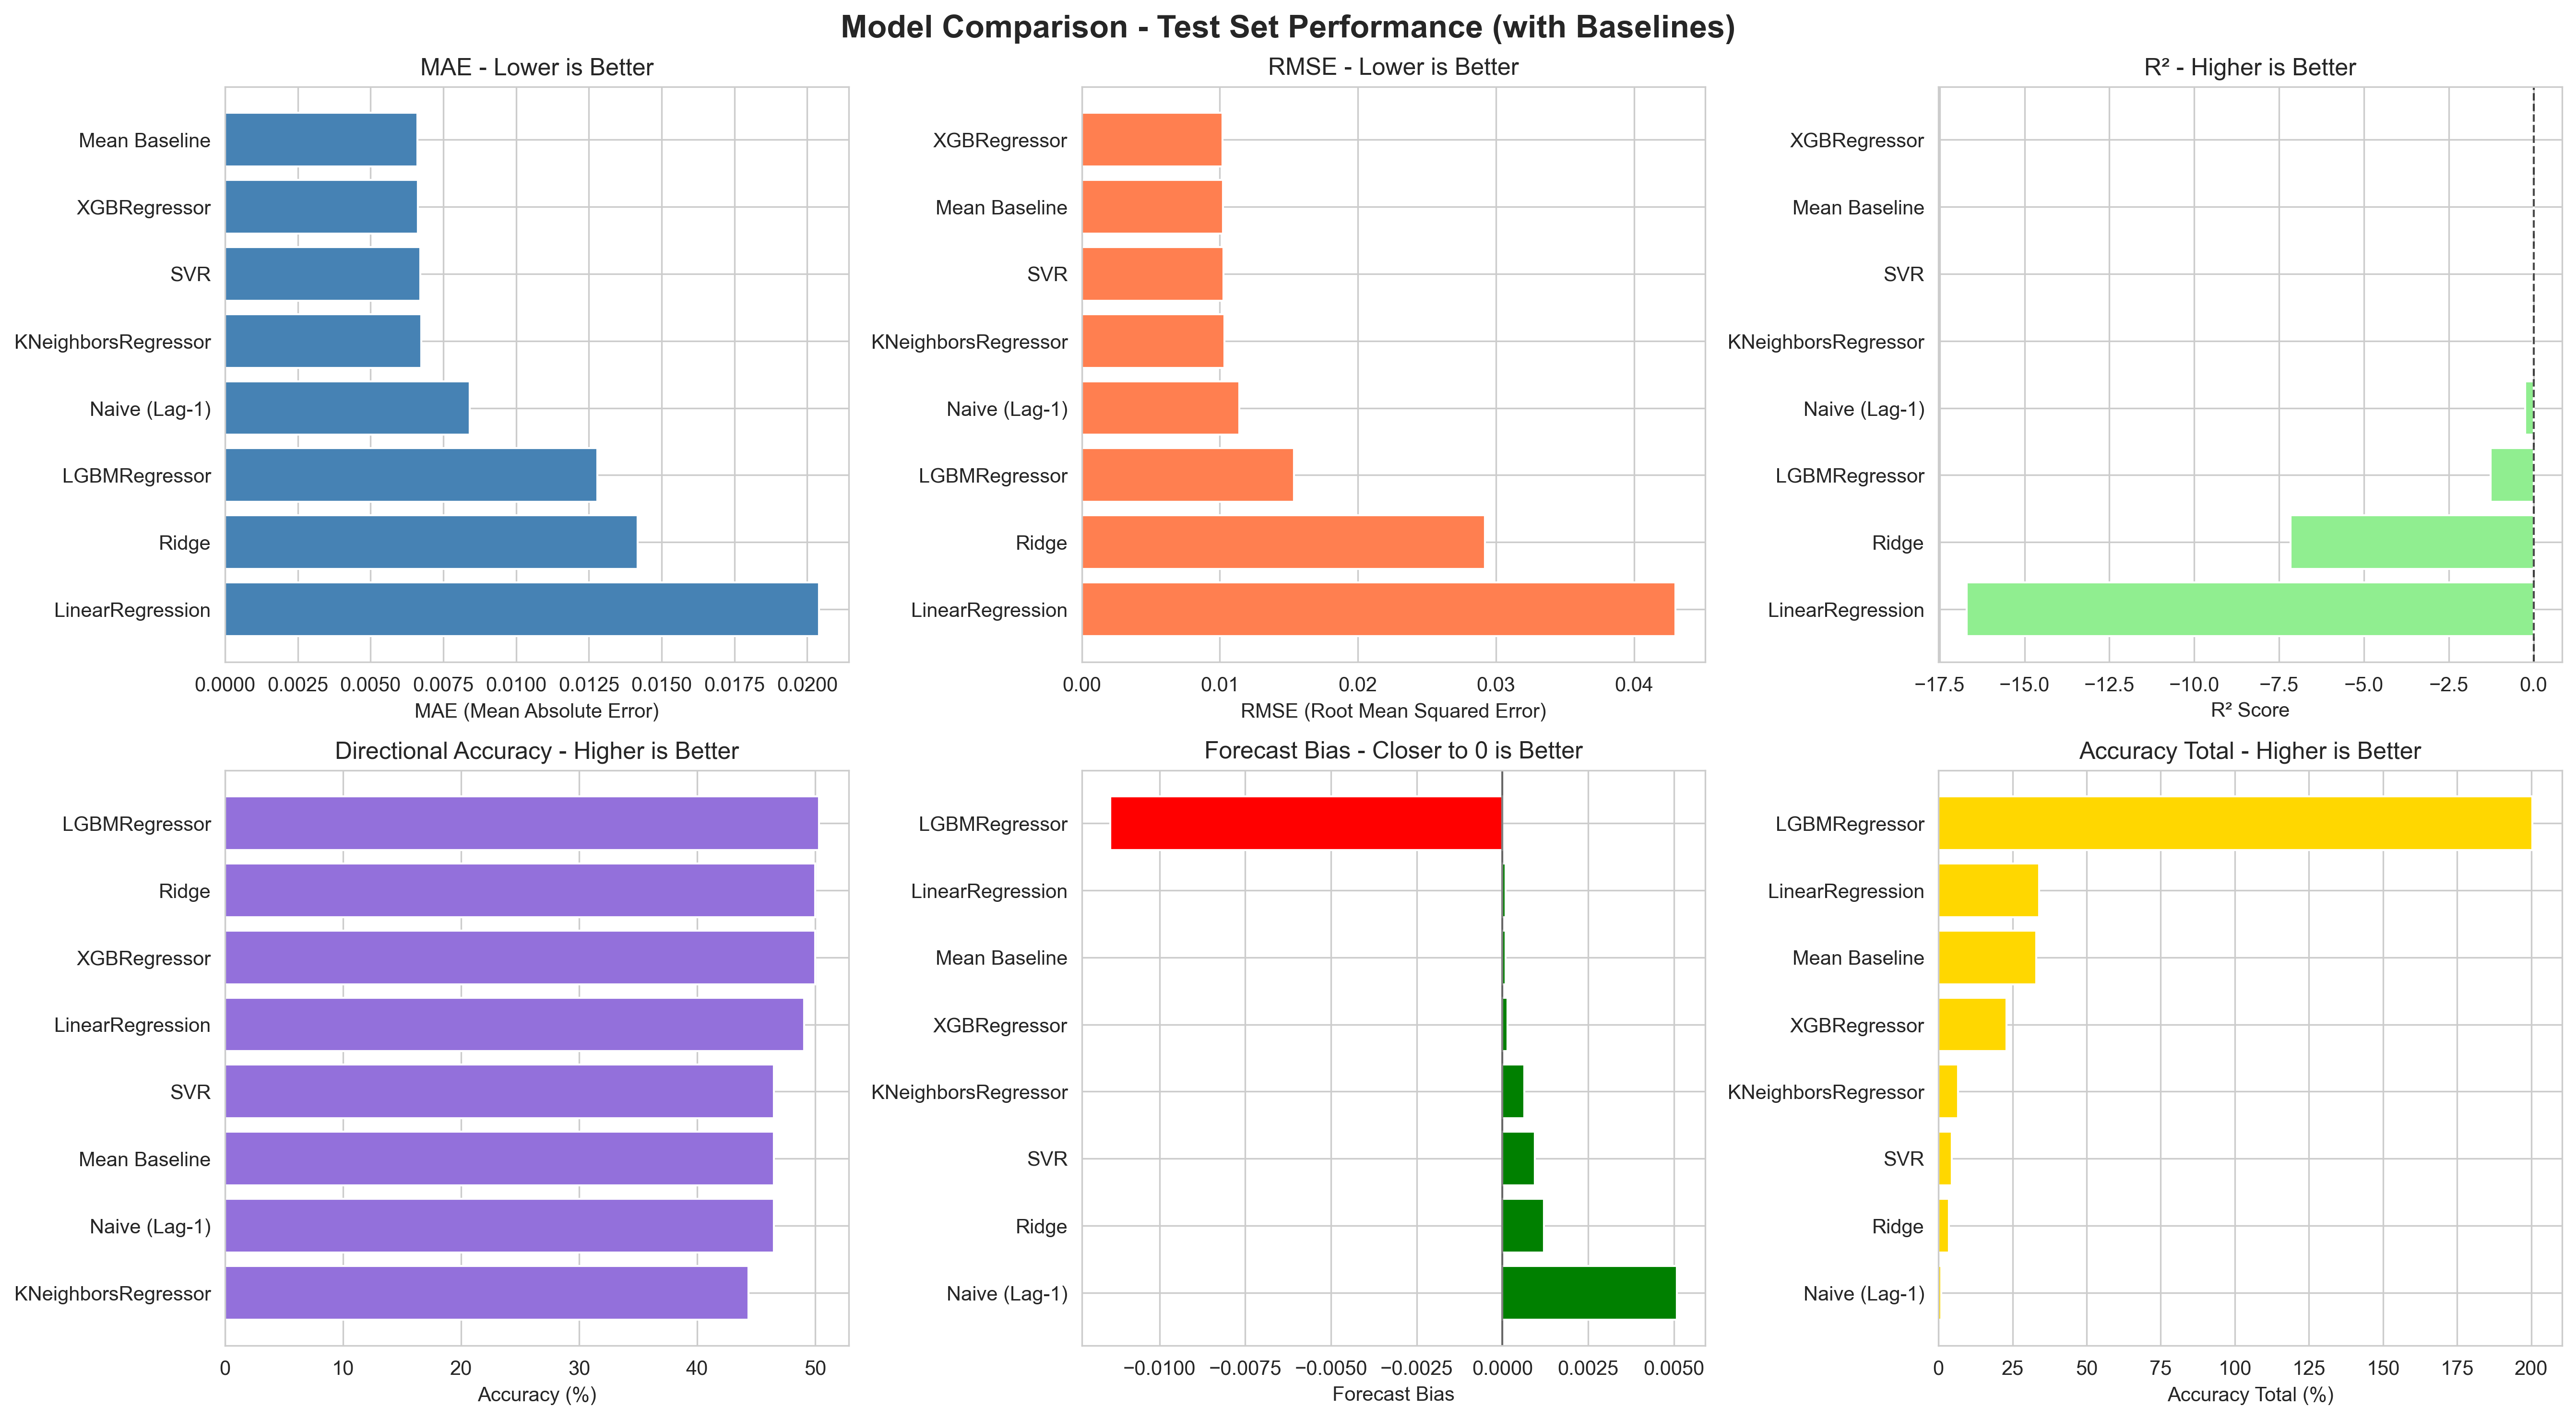
\includegraphics[width=0.9\linewidth]{./img/baseline_comparison_one_step_res_1h.png}
	\caption{Vergleich verschiedener Modelle auf den Testdaten.
	Auf der X-Achse sind verschiedene Algorithmen aufgetragen, die Y-Achse zeigt die jeweilige Richtungsgenauigkeit.
	Auffällig ist, dass alle Modelle um die gestrichelte 50\%-Linie schwanken, was die Schwierigkeit einer Richtungsbeurteilung verdeutlicht.}
    \label{fig:model_comp}
\end{figure}

Die grafische Auswertung verdeutlicht, dass keines der Basismodelle eine Richtungsgenauigkeit erzielt, die deutlich über dem Zufallsniveau liegt.
Technisch lässt sich dies darauf zurückführen, dass die Modelle Schwierigkeiten haben, die Zusammenhänge des Rohstoffmarktes allein aus den historischen Features zu extrahieren.

\subsection{Deep-Learning-Modelle und multi-temporale Analyse}
In der tiefergehenden Analyse des Deep-Learning-Verfahren (LSTM) werden die Vorhersagen der logarithmischen Renditen betrachtet.
Abbildung \ref{fig:daily_price_change} visualisiert die vorhergesagte Preisänderungen im Zeitverlauf.

\begin{figure}[hpt!]
\centering
	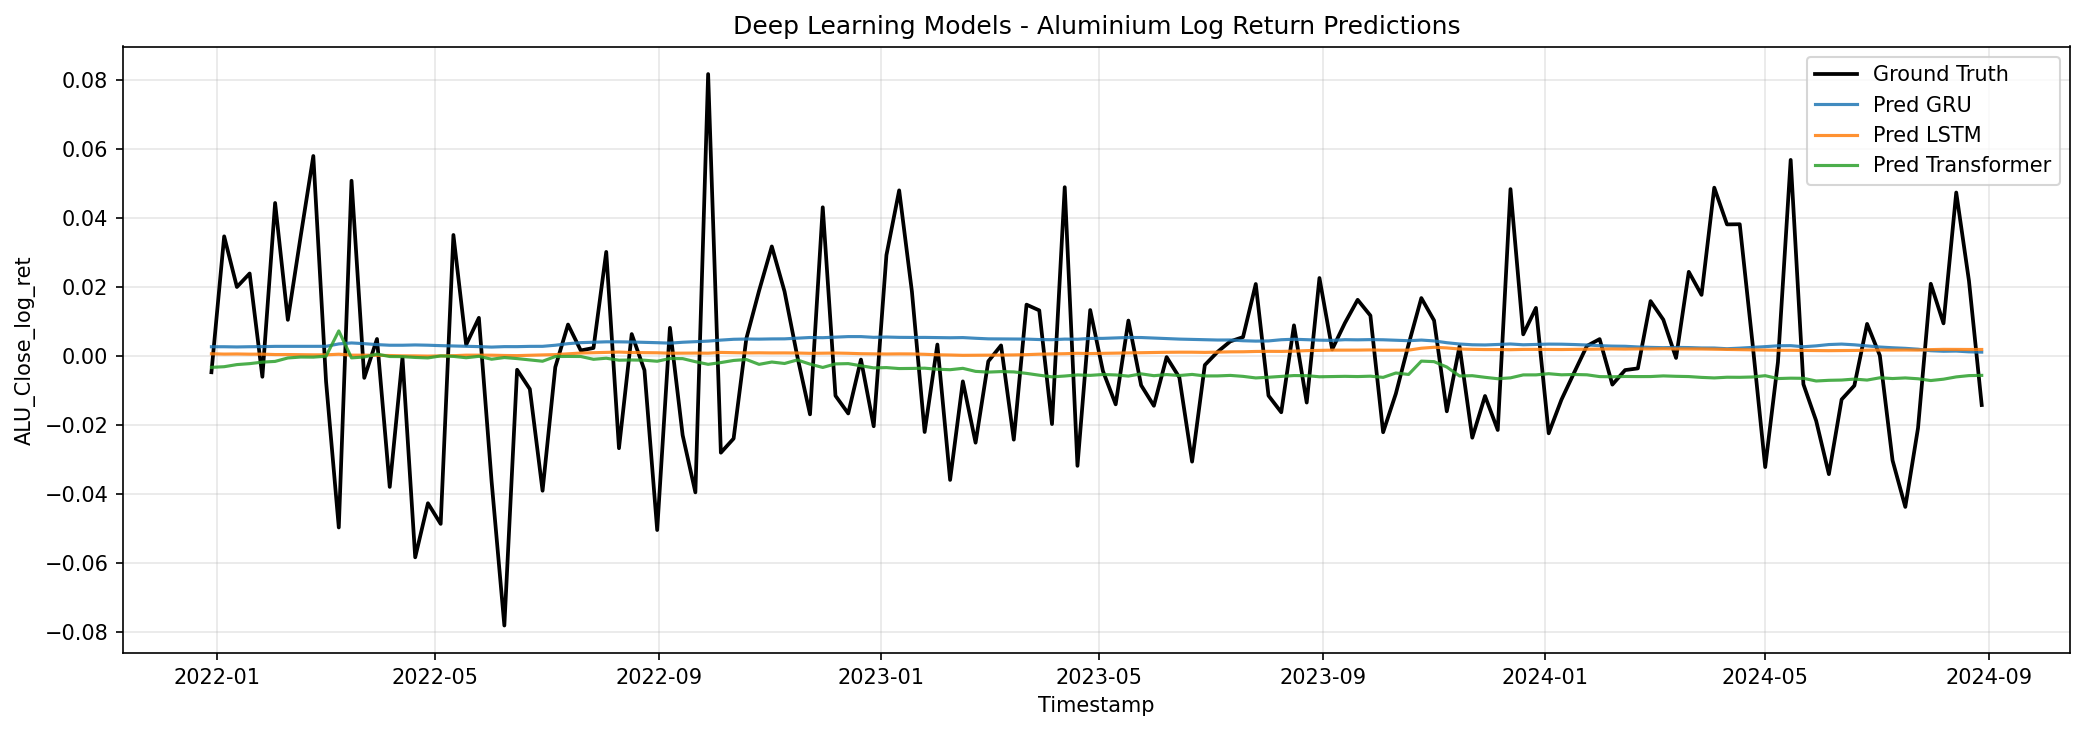
\includegraphics[width=0.9\linewidth]{./img/dl_models_test_predictions.png}
	\caption{Prognose der täglichen Preisänderung ($h=1$).
	Die X-Achse stellt den Zeitverlauf dar, die Y-Achse die logarithmische Rendite.
	Die farbigen Linien (Modelle) zeigen deutlich geringere Amplituden als die schwarze Linie (Wahrheit).
	Dies deutet auf eine vorsichtige Strategie des Modells hin, das nur kleine Änderungen vorhersagt.}
    \label{fig:daily_price_change}
\end{figure}

Wird diese Vorhersage auf das absolute Preisniveau in USD transformiert, ergibt sich die Darstellung in Abbildung \ref{fig:daily_price_pred}.
Hierbei wird die Vorhersage des Modells direkt gegen den realen Preis geplottet.

\begin{figure}[hpt!]
\centering
	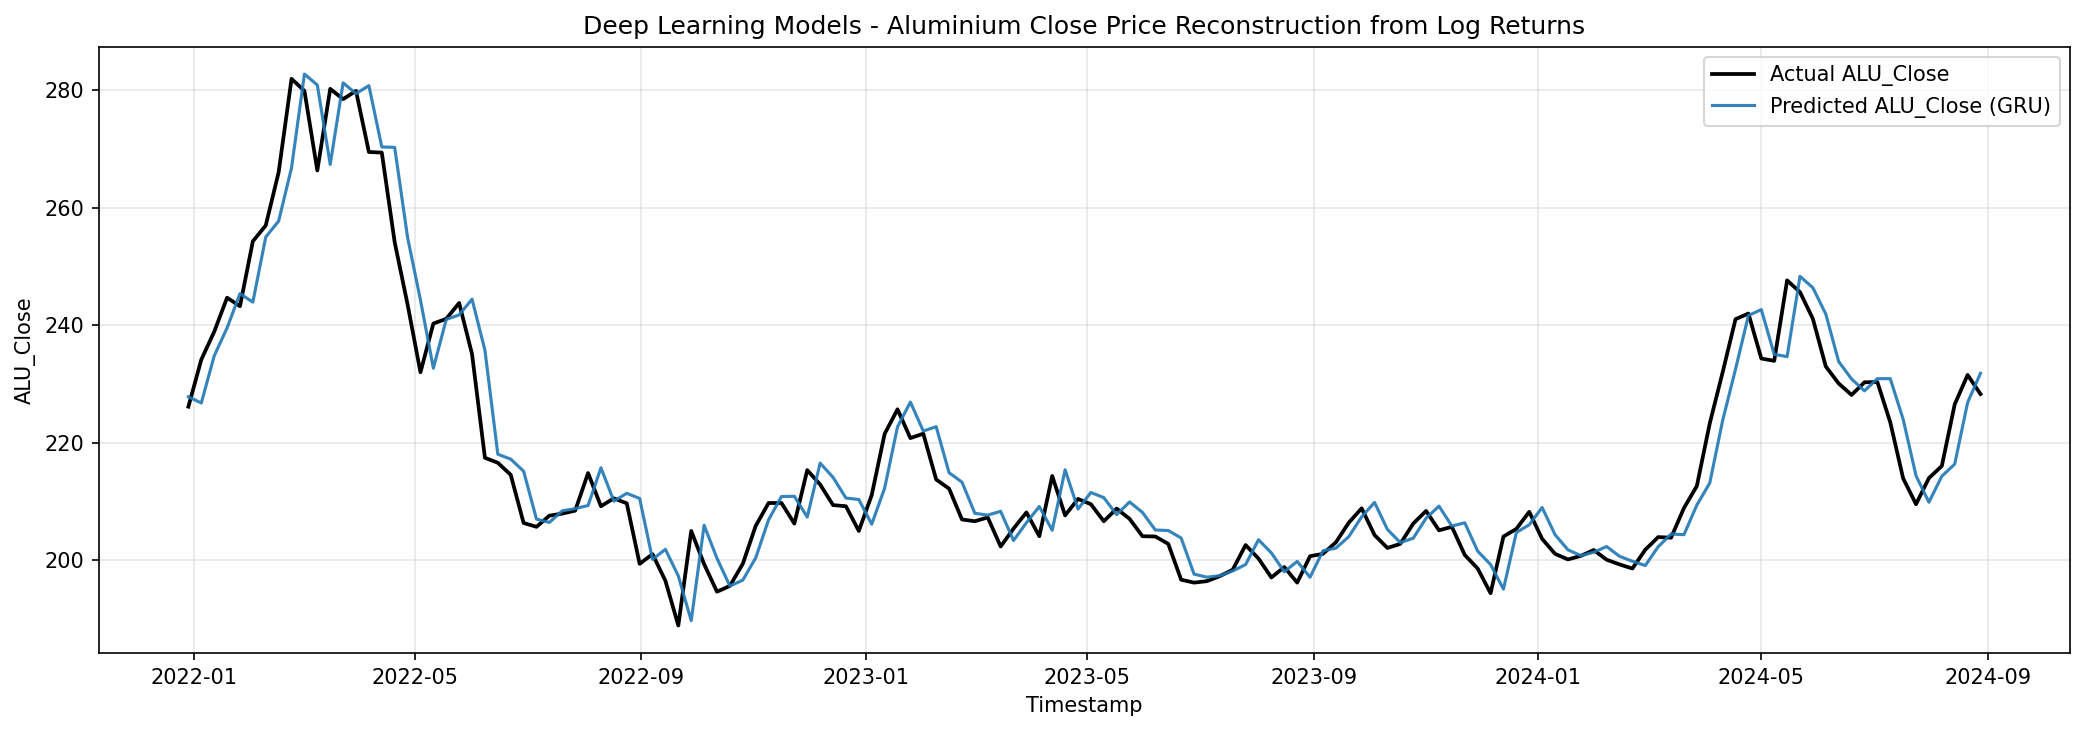
\includegraphics[width=0.9\linewidth]{./img/dl_models_test_price_predictions.png}
	\caption{Preisprognose im Vergleich zum realen Verlauf.
	Die blaue Linie repräsentiert den tatsächlichen Preis, die rote Linie die Modellvorhersage.
	Der Detailausschnitt zeigt, dass die rote Kurve der blauen fast identisch folgt, jedoch um genau einen Zeitschritt nach rechts verschoben ist.
	Das Modell nutzt den heutigen Preis als Schätzung für morgen (Lag-Effekt).}
    \label{fig:daily_price_pred}
\end{figure}

Dieses Verhalten zeigt darauf hin, dass das Modell zwar die aktuelle Preisregion korrekt identifiziert, aber keine echten Signale für die unmittelbare Zukunft generiert.
Für den Anwender bedeutet dies, dass das Modell den aktuellen Status einfach nur repliziert.

\subsection{Langzeit-Prognose im Walk-Forward-Modus}
Um die Stabilität über längere Zeiträume zu prüfen, wird ein Walk-Forward-Test durchgeführt, bei dem das Modell mehrere Tage in die Zukunft blickt, ohne zwischendurch neue Daten zu erhalten.
Abbildung \ref{fig:price_pred} zeigt das Ergebnis für eine mehrwöchige Prognose.

\begin{figure}[hpt!]
\centering
	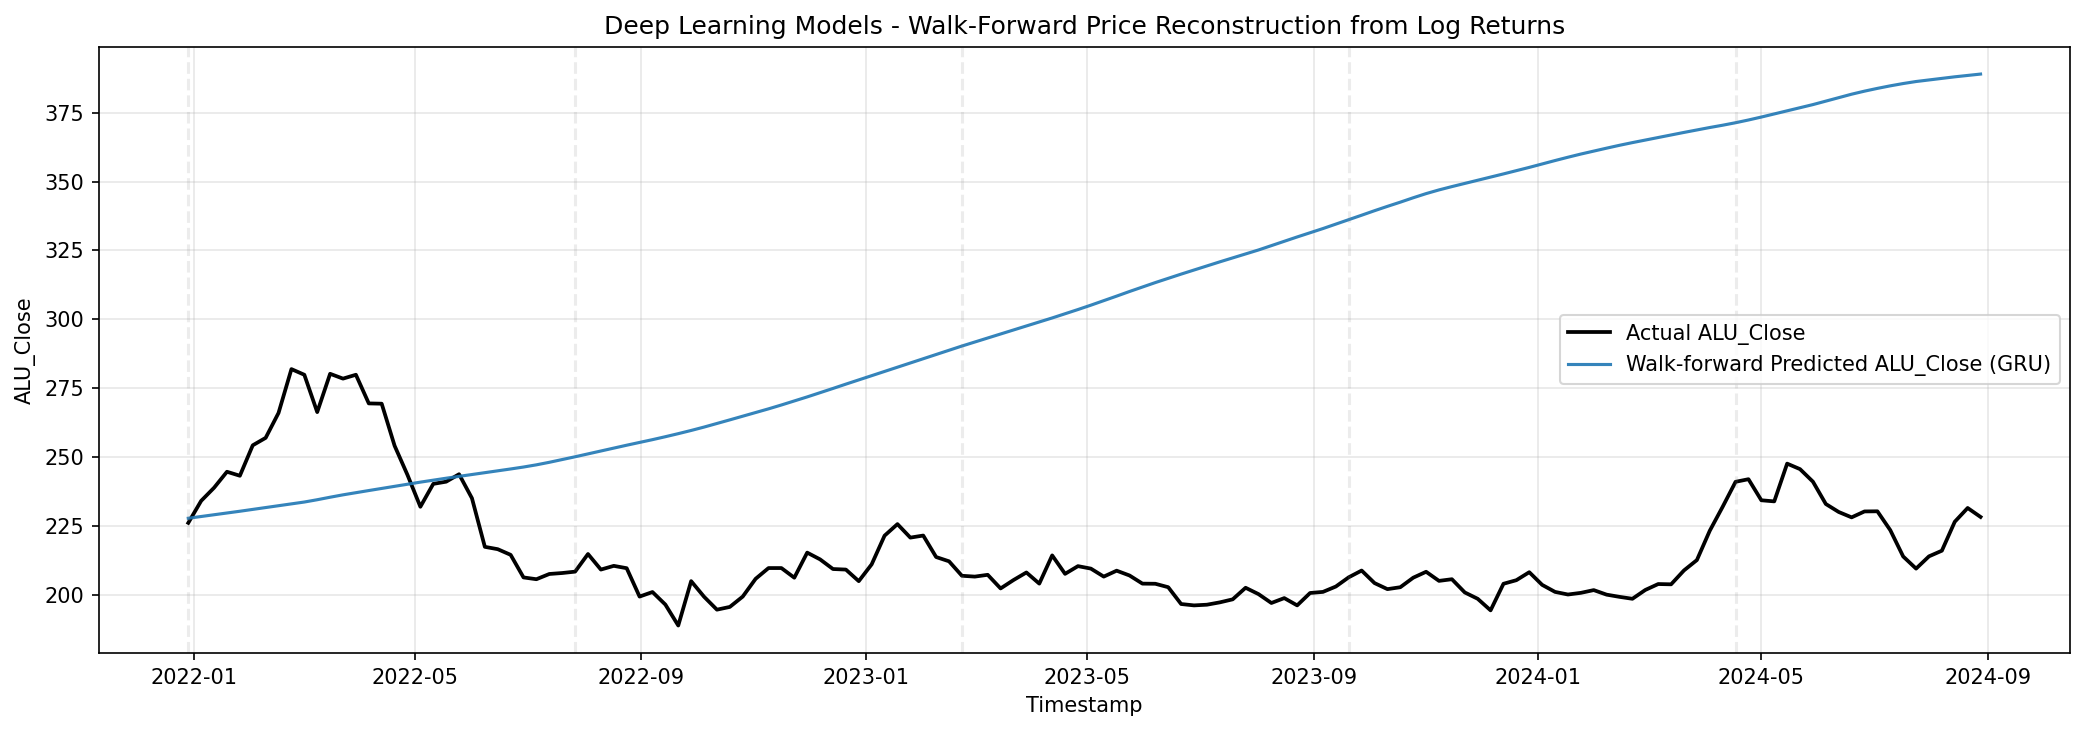
\includegraphics[width=0.9\linewidth]{./img/dl_models_walk_forward_price_plot.png}
	\caption{Mehrwöchige Preisvorhersage.
	Die X-Achse zeigt die Handelstage ab einem Startpunkt, die Y-Achse den Preis.
	Während die schwarze Linie (Realität) schwankt, zeigt die Modellvorhersage (farbige Linien) einen stetigen Drift nach oben oder unten.
	Da sich tägliche kleine Schätzfehler aufaddieren, entsteht eine zunehmende Lücke zum realen Preis.}
    \label{fig:price_pred}
\end{figure}

\subsection{Zusammenfassende Evaluation}
In Tabelle \ref{tab:results_lstm} sind die finalen Kennzahlen des Multi-Task-LSTMs zusammengefasst.
Diese Tabelle dient als Entscheidungsgrundlage für die Bewertung des Systems.

\begin{table}[h]
\centering
\caption{Quantitative Ergebnisse des Multi-Task-LSTMs}
\label{tab:results_lstm}
\begin{tabular}{lccccc}
\hline
\textbf{Horizont} & \textbf{$R^2$} & \textbf{MAE} & \textbf{RMSE} & \textbf{Dir. Acc.} & \textbf{Coverage@95\%} \\ \hline
1 Tag (h=1)        & 0,0043         & 0,0068       & 0,0102        & 51,1\,\%           & 90,8\,\%               \\
5 Tage (h=5)       & -0,0510        & 0,0185       & 0,0244        & 48,3\,\%           & 73,2\,\%               \\
21 Tage (h=21)     & -0,0795        & 0,0392       & 0,0514        & 50,3\,\%           & 56,0\,\%               \\ \hline
\end{tabular}
\end{table}

Abbildung \ref{fig:finale_testerg} fasst diese Metriken grafisch zusammen und erlaubt einen schnellen Überblick über die Abhängigkeit zwischen Vorhersagedauer und Modellpräzision.

\begin{figure}[hpt!]
\centering
	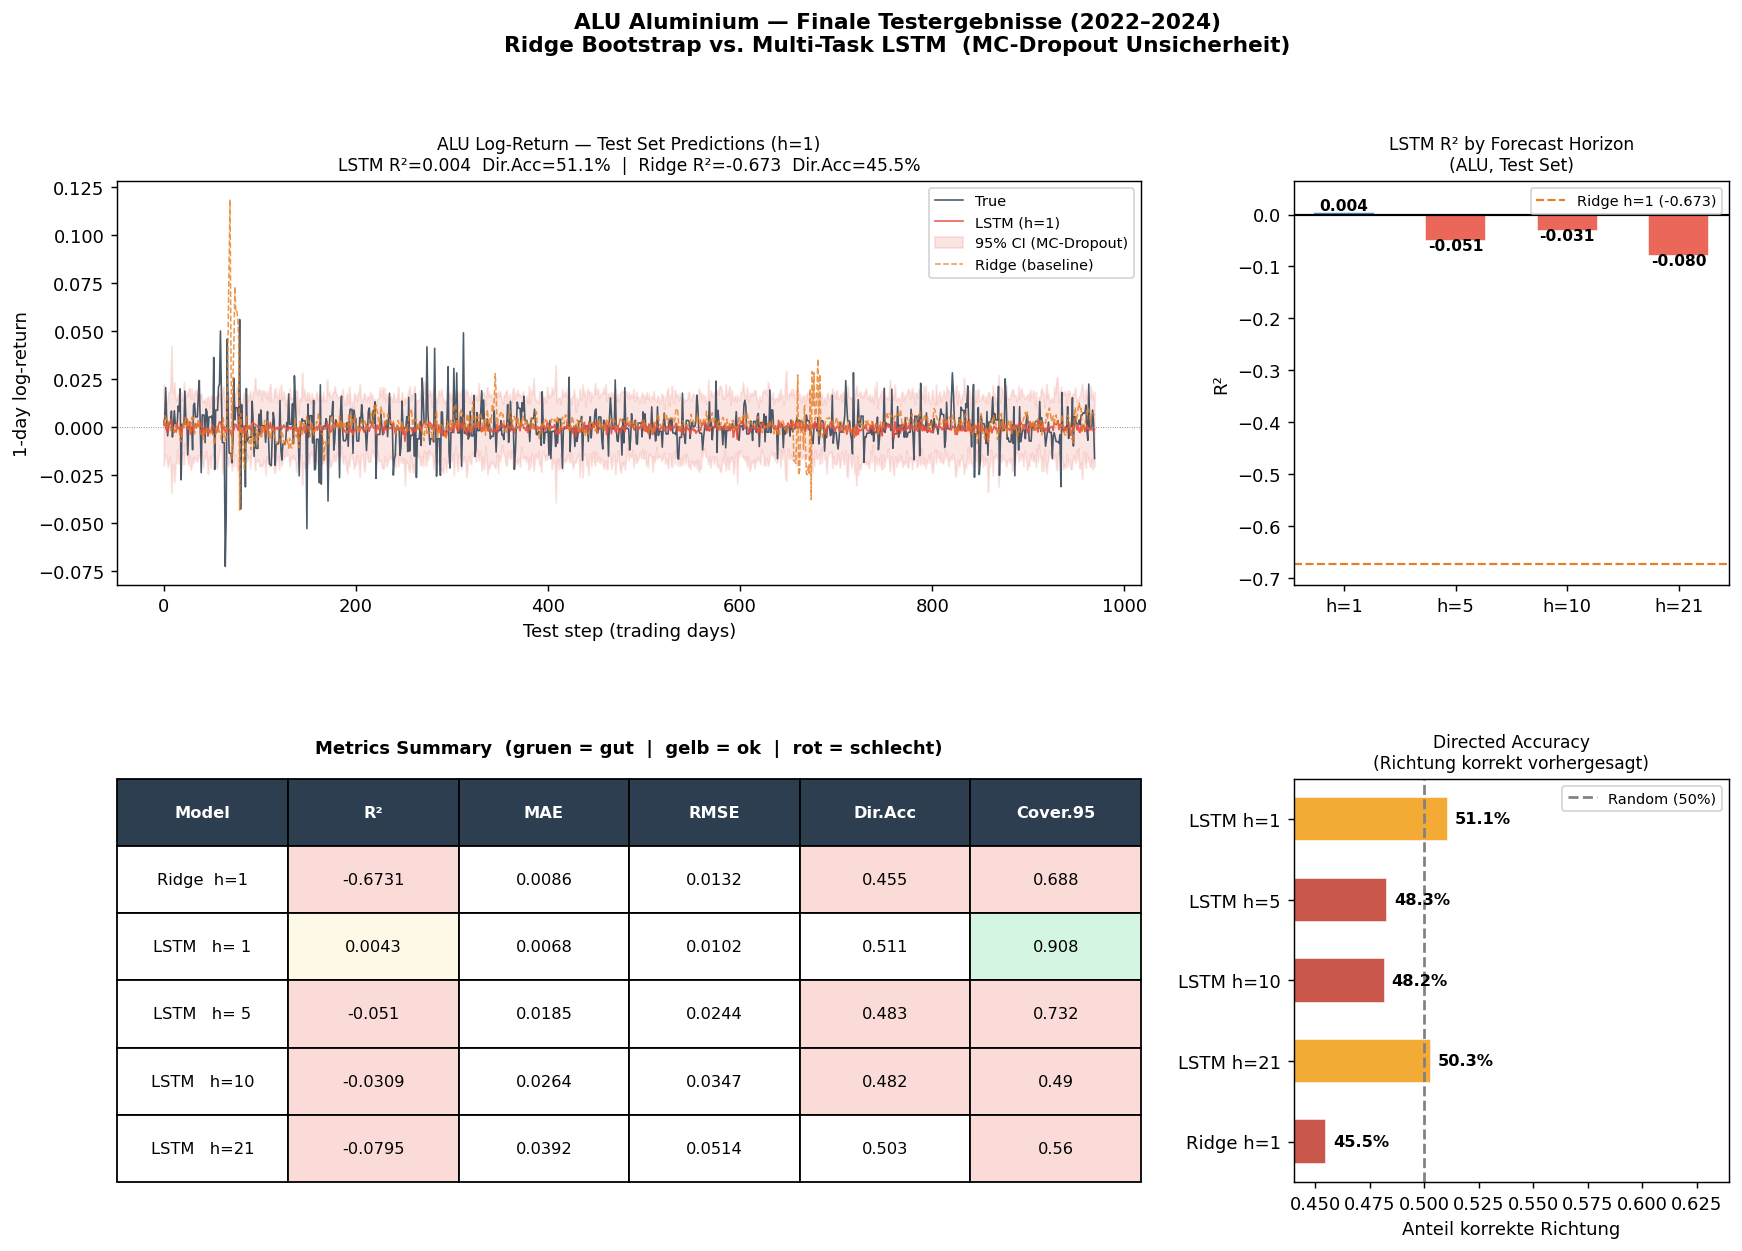
\includegraphics[width=0.9\linewidth]{./img/final_test_evaluation.png}
	\caption{Zusammenfassende Evaluation.
	Die obere Grafik zeigt die Vorhersagefehler über den Testzeitraum.
	Die Balkendiagramme unten vergleichen $R^2$-Werte und Richtungsgenauigkeit für verschiedene Horizonte.
	Es wird deutlich, dass die Vorhersagequalität mit zunehmendem zeitlichen Abstand zum aktuellen Tag abnimmt.}
    \label{fig:finale_testerg}
\end{figure}

